\chapter{Aikavaativuus}

\index{aikavaativuus@aikavaativuus}

Kisakoodauksessa oleellinen asia on algoritmien tehokkuus.
Yleensä on helppoa suunnitella algoritmi,
joka ratkaisee tehtävän hitaasti,
mutta todellinen vaikeus piilee siinä,
kuinka keksiä nopeasti toimiva algoritmi.
Jos algoritmi on liian hidas, se tuottaa vain
osan pisteistä tai ei pisteitä lainkaan.

\key{Aikavaativuus} on kätevä tapa arvioida,
kuinka nopeasti algoritmi toimii.
Se esittää algoritmin tehokkuuden funktiona,
jonka parametrina on syötteen koko.
Aikavaativuuden avulla algoritmista voi päätellä ennen koodaamista,
onko se riittävän tehokas tehtävän ratkaisuun.

\section{Laskusäännöt}

Algoritmin aikavaativuus merkitään $O(\cdots)$,
jossa kolmen pisteen tilalla
on kaava, joka kuvaa algoritmin ajankäyttöä.
Yleensä muuttuja $n$ esittää syötteen kokoa.
Esimerkiksi jos algoritmin syötteenä on taulukko lukuja,
$n$ on lukujen määrä,
ja jos syötteenä on merkkijono,
$n$ on merkkijonon pituus.

\subsubsection*{Silmukat}

Algoritmin ajankäyttö johtuu usein
pohjimmiltaan silmukoista,
jotka käyvät syötettä läpi.
Mitä enemmän sisäkkäisiä silmukoita
algoritmissa on, sitä hitaampi se on.
Jos sisäkkäisiä silmukoita on $k$,
aikavaativuus on $O(n^k)$.

Esimerkiksi seuraavan koodin aikavaativuus on $O(n)$:
\begin{lstlisting}
for (int i = 1; i <= n; i++) {
    // koodia
}
\end{lstlisting}

Vastaavasti seuraavan koodin aikavaativuus on $O(n^2)$:
\begin{lstlisting}
for (int i = 1; i <= n; i++) {
    for (int j = 1; j <= n; j++) {
        // koodia
    }
}
\end{lstlisting}

\subsubsection*{Suuruusluokka}

Aikavaativuus ei kerro tarkasti,
montako kertaa silmukan sisällä oleva koodi suoritetaan,
vaan se kertoo vain suuruusluokan.
Esimerkiksi seuraavissa esimerkeissä silmukat
suoritetaan $3n$, $n+5$ ja $\lfloor n/2 \rfloor$ kertaa,
mutta kunkin koodin aikavaativuus on sama $O(n)$.

\begin{lstlisting}
for (int i = 1; i <= 3*n; i++) {
    // koodia
}
\end{lstlisting}

\begin{lstlisting}
for (int i = 1; i <= n+5; i++) {
    // koodia
}
\end{lstlisting}

\begin{lstlisting}
for (int i = 1; i <= n; i += 2) {
    // koodia
}
\end{lstlisting}

Seuraavan koodin aikavaativuus on puolestaan $O(n^2)$:

\begin{lstlisting}
for (int i = 1; i <= n; i++) {
    for (int j = i+1; j <= n; j++) {
        // koodia
    }
}
\end{lstlisting}

\subsubsection*{Peräkkäisyys}

Jos koodissa on peräkkäisiä osia,
kokonaisaikavaativuus on suurin yksittäisen
osan aikavaativuus.
Tämä johtuu siitä, että koodin hitain
vaihe on yleensä koodin pullonkaula
ja muiden vaiheiden merkitys on pieni.

Esimerkiksi seuraava koodi muodostuu
kolmesta osasta,
joiden aikavaativuudet ovat $O(n)$, $O(n^2)$ ja $O(n)$.
Niinpä koodin aikavaativuus on $O(n^2)$.

\begin{lstlisting}
for (int i = 1; i <= n; i++) {
    // koodia
}
for (int i = 1; i <= n; i++) {
    for (int j = 1; j <= n; j++) {
        // koodia
    }
}
for (int i = 1; i <= n; i++) {
    // koodia
}
\end{lstlisting}

\subsubsection*{Monta muuttujaa}

Joskus syötteessä on monta muuttujaa,
jotka vaikuttavat aikavaativuuteen.
Tällöin myös aikavaativuuden kaavassa esiintyy
monta muuttujaa.

Esimerkiksi seuraavan koodin
aikavaativuus on $O(nm)$:

\begin{lstlisting}
for (int i = 1; i <= n; i++) {
    for (int j = 1; j <= m; j++) {
        // koodia
    }
}
\end{lstlisting}

\subsubsection*{Rekursio}

Rekursiivisen funktion aikavaativuuden
määrittää, montako kertaa funktiota kutsutaan yhteensä
ja mikä on yksittäisen kutsun aikavaativuus.
Kokonais\-aikavaativuus saadaan kertomalla
nämä arvot toisillaan.

Tarkastellaan esimerkiksi seuraavaa funktiota:
\begin{lstlisting}
void f(int n) {
    if (n == 1) return;
    f(n-1);
}
\end{lstlisting}
Kutsu $\texttt{f}(n)$ aiheuttaa yhteensä $n$ funktiokutsua,
ja jokainen funktiokutsu vie aikaa $O(1)$,
joten aikavaativuus on $O(n)$.

Tarkastellaan sitten seuraavaa funktiota:
\begin{lstlisting}
void g(int n) {
    if (n == 1) return;
    g(n-1);
    g(n-1);
}
\end{lstlisting}
Tässä tapauksessa funktio haarautuu kahteen osaan,
joten kutsu $\texttt{g}(n)$ aiheuttaa kaikkiaan seuraavat kutsut:
\begin{center}
\begin{tabular}{rr}
kutsu & kerrat \\
\hline
$\texttt{g}(n)$ & 1 \\
$\texttt{g}(n-1)$ & 2 \\
$\cdots$ & $\cdots$ \\
$\texttt{g}(1)$ & $2^{n-1}$ \\
\end{tabular}
\end{center}
Tämän perusteella kutsun $\texttt{g}(n)$ aikavaativuus on
\[1+2+4+\cdots+2^{n-1} = 2^n-1 = O(2^n).\]

\section{Vaativuusluokkia}

\index{vaativuusluokka@vaativuusluokka}

Usein esiintyviä vaativuusluokkia ovat seuraavat:

\begin{description}
\item[$O(1)$]
\index{vakioaikainen algoritmi@vakioaikainen algoritmi}
\key{Vakioaikainen} algoritmi
käyttää saman verran aikaa minkä tahansa
syötteen käsittelyyn,
eli algoritmin nopeus ei riipu syötteen koosta.
Tyypillinen vakioaikainen algoritmi on suora kaava
vastauksen laskemiseen.

\item[$O(\log n)$]
\index{logaritminen algoritmi@logaritminen algoritmi}
\key{Logaritminen} aikavaativuus
syntyy usein siitä, että algoritmi
puolittaa syötteen koon joka askeleella.
Logaritmi $\log_2 n$ näet ilmaisee, montako
kertaa luku $n$ täytyy puolittaa,
ennen kuin tuloksena on 1.

\item[$O(\sqrt n)$]

Tällainen algoritmi sijoittuu
aikavaativuuksien $O(\log n)$ ja $O(n)$ välimaastoon.
Neliöjuuren erityinen ominaisuus on,
että $\sqrt n = n/\sqrt n$, joten neliöjuuri
osuu tietyllä tavalla syötteen puoliväliin.

\item[$O(n)$]
\index{lineaarinen algoritmi@lineaarinen algoritmi}
\key{Lineaarinen} algoritmi käy syötteen läpi
kiinteän määrän kertoja.
Tämä on usein paras mahdollinen aikavaativuus,
koska yleensä syöte täytyy käydä
läpi ainakin kerran,
ennen kuin algoritmi voi ilmoittaa vastauksen.

\item[$O(n \log n)$]

Tämä aikavaativuus viittaa usein
syötteen järjestämiseen,
koska tehokkaat järjestämisalgoritmit toimivat
ajassa $O(n \log n)$.
Toinen mahdollisuus on, että algoritmi
käyttää tietorakennetta,
jonka operaatiot ovat $O(\log n)$-aikaisia.

\item[$O(n^2)$]
\index{nelizllinen algoritmi@neliöllinen algoritmi}
\key{Neliöllinen} aikavaativuus voi syntyä
siitä, että algoritmissa on 
kaksi sisäkkäistä silmukkaa.
Neliöllinen algoritmi voi käydä läpi kaikki
tavat valita joukosta kaksi alkiota.

\item[$O(n^3)$]
\index{kuutiollinen algoritmi@kuutiollinen algoritmi}
\key{Kuutiollinen} aikavaativuus voi syntyä siitä,
että algoritmissa on 
kolme sisäkkäistä silmukkaa.
Kuutiollinen algoritmi voi käydä läpi kaikki
tavat valita joukosta kolme alkiota.

\item[$O(2^n)$]

Tämä aikavaativuus tarkoittaa usein,
että algoritmi käy läpi kaikki syötteen osajoukot.
Esimerkiksi joukon $\{1,2,3\}$ osajoukot ovat
$\emptyset$, $\{1\}$, $\{2\}$, $\{3\}$, $\{1,2\}$,
$\{1,3\}$, $\{2,3\}$, $\{1,2,3\}$,
missä $\emptyset$ on tyhjä joukko.

\item[$O(n!)$]

Tämä aikavaativuus voi syntyä siitä,
että algoritmi käy läpi kaikki syötteen permutaatiot.
Esimerkiksi joukon $\{1,2,3\}$ permutaatiot ovat
$(1,2,3)$, $(1,3,2)$, $(2,1,3)$, $(2,3,1)$,
$(3,1,2)$ sekä $(3,2,1)$.

\end{description}

\index{polynominen algoritmi@polynominen algoritmi}
Algoritmi on \key{polynominen},
jos sen aikavaativuus on korkeintaan $O(n^k)$,
kun $k$ on vakio.
Edellä mainituista aikavaativuuksista
kaikki paitsi $O(2^n)$ ja $O(n!)$
ovat polynomisia.
Käytännössä vakio $k$ on yleensä pieni,
minkä ansiosta
polynomisuus kuvastaa sitä,
että algoritmi on \emph{tehokas}.
\index{NP-vaikea ongelma}

Useimmat tässä kirjassa esitettävät algoritmit
ovat polynomisia.
Silti on paljon ongelmia, joihin ei tunneta
polynomista algoritmia eli ongelmaa ei osata
ratkaista tehokkaasti.
\key{NP-vaikeat} ongelmat ovat
tärkeä joukko ongelmia,
joihin ei tiedetä polynomista algoritmia.

\section{Tehokkuuden arviointi}

Aikavaativuuden hyötynä on,
että sen avulla voi arvioida ennen algoritmin
toteuttamista, onko algoritmi riittävän nopea
tehtävän ratkaisemiseen.
Lähtökohtana arviossa on, että nykyaikainen tietokone
pystyy suorittamaan sekunnissa joitakin
satoja miljoonia koodissa olevia komentoja.

Oletetaan esimerkiksi, että tehtävän aikaraja on 
yksi sekunti ja syötteen koko on $n=10^5$.
Jos algoritmin aikavaativuus on $O(n^2)$,
algoritmi suorittaa noin $(10^5)^2=10^{10}$ komentoa.
Tähän kuluu aikaa arviolta kymmeniä sekunteja,
joten algoritmi vaikuttaa liian hitaalta tehtävän ratkaisemiseen.

Käänteisesti syötteen koosta voi päätellä,
kuinka tehokasta algoritmia tehtävän laatija odottaa
ratkaisijalta.
Seuraavassa taulukossa on joitakin hyödyllisiä arvioita,
jotka olettavat, että tehtävän aikaraja on yksi sekunti.

\begin{center}
\begin{tabular}{ll}
syötteen koko ($n$) & haluttu aikavaativuus \\
\hline
$n \le 10^{18}$ & $O(1)$ tai $O(\log n)$ \\
$n \le 10^{12}$ & $O(\sqrt n)$ \\
$n \le 10^6$ & $O(n)$ tai $O(n \log n)$ \\
$n \le 5000$ & $O(n^2)$ \\
$n \le 500$ & $O(n^3)$ \\
$n \le 25$ & $O(2^n)$ \\
$n \le 10$ & $O(n!)$ \\
\end{tabular}
\end{center}

Esimerkiksi jos syötteen koko on $n=10^5$,
tehtävän laatija odottaa luultavasti
algoritmia, jonka aikavaativuus on $O(n)$ tai $O(n \log n)$.
Tämä tieto helpottaa algoritmin suunnittelua,
koska se rajaa pois monia lähestymistapoja,
joiden tuloksena olisi hitaampi aikavaativuus.

Aikavaativuus ei kerro kuitenkaan kaikkea algoritmin
tehokkuudesta, koska se kätkee toteutuksessa olevat
vakiokertoimet. Esimerkiksi aikavaativuuden $O(n)$
algoritmi voi tehdä käytännössä $n/2$ tai $5n$ operaatiota.
Tällä on merkittävä vaikutus algoritmin
todelliseen ajankäyttöön.

\section{Suurin alitaulukon summa}

\index{suurin alitaulukon summa@suurin alitaulukon summa}

Usein ohjelmointitehtävän ratkaisuun on monta
luontevaa algoritmia, joiden aikavaativuudet eroavat.
Tutustumme seuraavaksi klassiseen ongelmaan,
jonka suoraviivaisen ratkaisun aikavaativuus on $O(n^3)$,
mutta algoritmia parantamalla aikavaativuudeksi
tulee ensin $O(n^2)$ ja lopulta $O(n)$.

Annettuna on taulukko, jossa on $n$ kokonaislukua
$x_1,x_2,\ldots,x_n$, ja tehtävänä on etsiä
taulukon \key{suurin alitaulukon summa}
eli mahdollisimman suuri summa
taulukon yhtenäisellä välillä.
Tehtävän kiinnostavuus on siinä, että taulukossa
saattaa olla negatiivisia lukuja.
Esimerkiksi taulukossa
\begin{center}
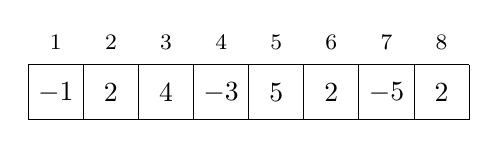
\begin{tikzpicture}[scale=0.7]
\draw (0,0) grid (8,1);

\node at (0.5,0.5) {$-1$};
\node at (1.5,0.5) {$2$};
\node at (2.5,0.5) {$4$};
\node at (3.5,0.5) {$-3$};
\node at (4.5,0.5) {$5$};
\node at (5.5,0.5) {$2$};
\node at (6.5,0.5) {$-5$};
\node at (7.5,0.5) {$2$};

\footnotesize
\node at (0.5,1.4) {$1$};
\node at (1.5,1.4) {$2$};
\node at (2.5,1.4) {$3$};
\node at (3.5,1.4) {$4$};
\node at (4.5,1.4) {$5$};
\node at (5.5,1.4) {$6$};
\node at (6.5,1.4) {$7$};
\node at (7.5,1.4) {$8$};
\end{tikzpicture}
\end{center}
\begin{samepage}
suurimman summan $10$ tuottaa seuraava alitaulukko:
\begin{center}
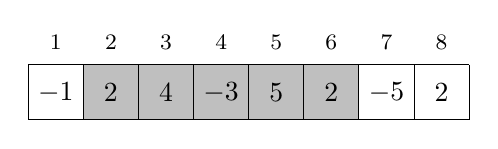
\begin{tikzpicture}[scale=0.7]
\fill[color=lightgray] (1,0) rectangle (6,1);
\draw (0,0) grid (8,1);

\node at (0.5,0.5) {$-1$};
\node at (1.5,0.5) {$2$};
\node at (2.5,0.5) {$4$};
\node at (3.5,0.5) {$-3$};
\node at (4.5,0.5) {$5$};
\node at (5.5,0.5) {$2$};
\node at (6.5,0.5) {$-5$};
\node at (7.5,0.5) {$2$};

\footnotesize
\node at (0.5,1.4) {$1$};
\node at (1.5,1.4) {$2$};
\node at (2.5,1.4) {$3$};
\node at (3.5,1.4) {$4$};
\node at (4.5,1.4) {$5$};
\node at (5.5,1.4) {$6$};
\node at (6.5,1.4) {$7$};
\node at (7.5,1.4) {$8$};
\end{tikzpicture}
\end{center}
\end{samepage}


\subsubsection{Ratkaisu 1}

Suoraviivainen ratkaisu tehtävään on käydä
läpi kaikki tavat valita alitaulukko taulukosta,
laskea jokaisesta vaihtoehdosta lukujen summa
ja pitää muistissa suurinta summaa.
Seuraava koodi toteuttaa tämän algoritmin:

\begin{lstlisting}
int p = 0;
for (int a = 1; a <= n; a++) {
    for (int b = a; b <= n; b++) {
        int s = 0;
        for (int c = a; c <= b; c++) {
            s += x[c];
        }
        p = max(p,s);
    }
}
cout << p << "\n";
\end{lstlisting}

Koodi olettaa, että luvut on tallennettu taulukkoon \texttt{x},
jota indeksoidaan $1 \ldots n$.
Muuttujat $a$ ja $b$ valitsevat alitaulukon ensimmäisen
ja viimeisen luvun, ja alitaulukon summa lasketaan muuttujaan $s$.
Muuttujassa $p$ on puolestaan paras haun aikana löydetty summa.

Algoritmin aikavaativuus on $O(n^3)$, koska siinä on kolme
sisäkkäistä silmukkaa ja jokainen silmukka käy läpi $O(n)$ lukua.

\subsubsection{Ratkaisu 2}

Äskeistä ratkaisua on helppoa tehostaa hankkiutumalla
eroon sisimmästä silmukasta.
Tämä on mahdollista laskemalla summaa samalla,
kun alitaulukon oikea reuna liikkuu eteenpäin.
Tuloksena on seuraava koodi:

\begin{lstlisting}
int p = 0;
for (int a = 1; a <= n; a++) {
    int s = 0;
    for (int b = a; b <= n; b++) {
        s += x[b];
        p = max(p,s);
    }
}
cout << p << "\n";
\end{lstlisting}
Tämän muutoksen jälkeen koodin aikavaativuus on $O(n^2)$.

\subsubsection{Ratkaisu 3}

Yllättävää kyllä, tehtävään on olemassa myös
$O(n)$-aikainen ratkaisu eli koodista pystyy
karsimaan vielä yhden silmukan.
Ideana on laskea taulukon jokaiseen
kohtaan, mikä on suurin alitaulukon
summa, jos alitaulukko päättyy kyseiseen kohtaan
Tämän jälkeen ratkaisu tehtävään on suurin
näistä summista.

Tarkastellaan alitaulukon etsimistä,
kun valittuna on alitaulukon loppukohta $k$.
Vaihtoehtoja on kaksi:
\begin{enumerate}
\item Alitaulukossa on vain kohdassa $k$ oleva luku.
\item Alitaulukossa on ensin jokin kohtaan $k-1$ päättyvä alitaulukko
ja sen jälkeen kohdassa $k$ oleva luku.
\end{enumerate}

Koska tavoitteena on löytää alitaulukko,
jonka lukujen summa on suurin,
tapauksessa 2 myös kohtaan $k-1$ päättyvän
alitaulukon tulee olla sellainen,
että sen summa on suurin.
Niinpä tehokas ratkaisu syntyy käymällä läpi
kaikki alitaulukon loppukohdat järjestyksessä
ja laskemalla jokaiseen kohtaan suurin
mahdollinen kohtaan päättyvän alitaulukon summa.

Seuraava koodi toteuttaa ratkaisun:

\begin{lstlisting}
int p = 0, s = 0;
for (int k = 1; k <= n; k++) {
    s = max(x[k],s+x[k]);
    p = max(p,s);
}
cout << p << "\n";
\end{lstlisting}

Algoritmissa on vain yksi silmukka,
joka käy läpi taulukon luvut,
joten sen aikavaativuus on $O(n)$.
Tämä on myös paras mahdollinen aikavaativuus,
koska minkä tahansa algoritmin täytyy käydä
läpi ainakin kerran taulukon sisältö.

\subsubsection{Tehokkuusvertailu}

On kiinnostavaa tutkia, kuinka tehokkaita algoritmit
ovat käytännössä.
Seuraava taulukko näyttää, kuinka nopeasti äskeiset
ratkaisut toimivat eri $n$:n arvoilla
nykyaikaisella tietokoneella.

Jokaisessa testissä syöte on muodostettu satunnaisesti.
Ajankäyttöön ei ole laskettu syötteen lukemiseen
kuluvaa aikaa.

\begin{center}
\begin{tabular}{rrrr}
taulukon koko $n$ & ratkaisu 1 & ratkaisu 2 & ratkaisu 3 \\
\hline
$10^2$ & $0{,}0$ s & $0{,}0$ s & $0{,}0$ s \\
$10^3$ & $0{,}1$ s & $0{,}0$ s & $0{,}0$ s \\
$10^4$ & > $10,0$ s & $0{,}1$ s & $0{,}0$ s \\
$10^5$ & > $10,0$ s & $5{,}3$ s & $0{,}0$ s \\
$10^6$ & > $10,0$ s & > $10,0$ s & $0{,}0$ s \\
$10^7$ & > $10,0$ s & > $10,0$ s & $0{,}0$ s \\
\end{tabular}
\end{center}

Vertailu osoittaa,
että pienillä syötteillä kaikki algoritmit
ovat tehokkaita,
mutta suuremmat syötteet tuovat esille
merkittäviä eroja algoritmien suoritusajassa.
$O(n^3)$-aikainen ratkaisu 1 alkaa hidastua,
kun $n=10^3$, ja $O(n^2)$-aikainen ratkaisu 2
alkaa hidastua, kun $n=10^4$.
Vain $O(n)$-aikainen ratkaisu 3 selvittää
suurimmatkin syötteet salamannopeasti.
